\documentclass[a4paper]{article}
\usepackage[utf8]{inputenc}
\usepackage[russian,english]{babel}
\usepackage[T2A]{fontenc}
\usepackage[left=10mm, top=20mm, right=18mm, bottom=15mm, footskip=10mm]{geometry}
\usepackage{indentfirst}
\usepackage{amsmath,amssymb}
\usepackage[italicdiff]{physics}
\usepackage{graphicx}
\usepackage{caption}
\usepackage{float}
\renewcommand{\thefootnote}{\fnsymbol{footnote}}
\usepackage{tablefootnote}
\usepackage{footmisc}
\usepackage[parfill]{parskip}
\usepackage[utf8]{inputenc}\newcommand{\approxtext}[1]{\ensuremath{\stackrel{\text{#1}}{\approx}}}
\graphicspath{{images/}}
\DeclareGraphicsExtensions{.pdf,.png,.jpg}
\usepackage{wrapfig}
\captionsetup{labelformat=empty}
\usepackage{caption}
\captionsetup[figure]{name=Рисунок}
\captionsetup[table]{name=Таблица}
  
\title{\textbf{Отчет о выполненой лабораторной работе 2.2.3}}
\date{}
\author{Котляров Михаил, Б01-402}

\begin{document}

\maketitle
	
	\section{Введение}
	
	\textbf{Цель работы:} измерить коэффициент теплопроводности воздуха при атмосферном
давлении в зависимости от температуры.\\

	\textbf{Оборудование:} цилиндрическая колба с натянутой по оси нитью; термостат;
вольтметр и амперметр (цифровые мультиметры); источник
постоянного напряжения; магазин сопротивлений.
	
	\section{Теоретические сведения}
\textit{Теплопроводность} — это процесс передачи тепловой энергии от нагретых частей системы к холодным за счёт хаотического движения частиц среды (молекул, атомов и т.п.). В газах теплопроводность осуществляется за счёт  непосредственной передачи кинетической энергии от быстрых молекул к медленным при их столкновениях. Перенос тепла описывается законом Фурье, утверждающим, что плотность потока энергии 
\begin{equation*}
	\overline{q} = -k \nabla T,
	\eqno(1)
\end{equation*} где $k \left[ \dfrac{\text{Вт}}{\text{м} \cdot \text{К}} \right]$ - \textit{коэффициент теплопроводности}.
Среднее расстояние, на котором молекулы двигаются без столкновений, называется длиной свободного пробега. Будем обозначать эту величину $\lambda$.
Молекулярно-кинетическая теория дает следующую оценку для коэффициента теплопроводности газов:

\begin{equation*}
	k \sim \lambda \overline{\nu} \cdot n c_V \label{k},
	\eqno(2)
\end{equation*}
где $\lambda$  -  длина свободного пробега молекул газа, $\overline{\nu} = \sqrt{\frac{8k_{\text{Б}}T}{\pi m}}$ — средняя скорость их теплового движения, $n$ — концентрация (объёмная плотность) газа, $c_V = \frac{i}{2}k_{\text{Б}}$ - его теплоёмкость при постоянном объёме в расчёте на одну молекулу ($i$ — эффективное число степеней свободы молекулы). Длина свободного пробега может быть оценена как $\lambda = \frac{1}{\sigma n}$, где $\sigma$ — эффективное сечение столкновений молекул друг с другом. В модели частиц, как одинаковых твердых шариков $\sigma = \pi d^2$, где $d$ - диаметр шарика. Тогда из (2) видно, что k не зависит от плотности и определяется только температурой.
Рассматривая стационарную теплопроводность в цилиндрической геометрии, где пренебрегаются теплоотвод через торцы и перепад температур между нитью и стенками, а параметры газа считаются зависящами только от расстояния до оси системы, справедлива следущая формула
\begin{equation*}
	Q = \dfrac{2 \pi L}{\ln \dfrac{r_0}{r_1}} k  \cdot \Delta T 
	\eqno(3)
\end{equation*}
\clearpage
\begin{figure}[h!]
        \centering
        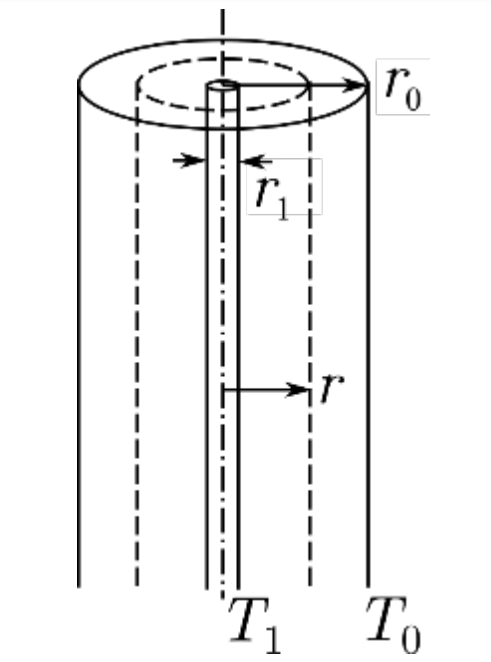
\includegraphics[scale=0.8]{Pictures/Cylinder.png}
        \caption{
        Рис. 1. Цилиндрическая установка
        }
 \end{figure} 

\section{Экспериментальная установка}
\begin{wrapfigure}{r}{0.4\textwidth}
        \begin{center}
            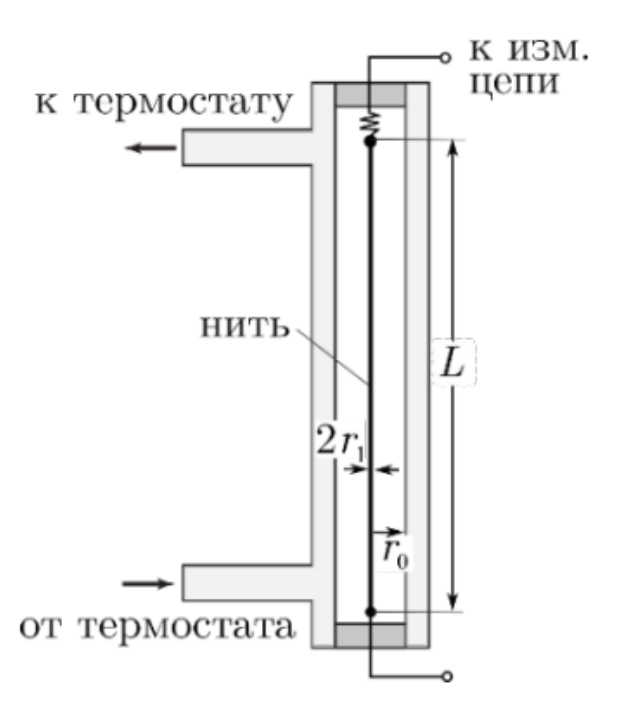
\includegraphics[width = 0.3\textwidth]{Pictures/ustanovka.png}
        \end{center}
        \textbf{\caption{Рис. 2. Схема установки}}
        \end{wrapfigure}
        Схема установки приведена на $\text{рис. 2.}$ На оси полой цилиндрической трубки с внутренним диаметром $2r_0\approx0,7\pm0,01$ см размещена металлическая нить диаметром $2r_1\approx0,05\pm0,003$ мм и длиной $L\approx40\pm0,2$ см (материал нити и точные геометрические размеры указаны в техническом описании установки). Полость трубки заполнена воздухом (полость через небольшое отверстие сообщается с атмосферой). Стенки трубки помещены в кожух, через которых пропускается вода из термостата, так что их температура $t_0$ поддерживается постоянной. Для предотвращения конвекции трубка расположена вертикально.

        Металлическая нить служит как источником тепла, так и датчиком температуры (термометром сопротивления). По пропускаемому через нить постоянному току $I$ и напряжению $U$ на ней вычисляется мощность нагрева по закону Джоуля–Ленца: $Q = UI$, и сопротивление нити по закону Ома: $R = \frac{U}{I}$.\\
\begin{figure}[h!]
        \centering
        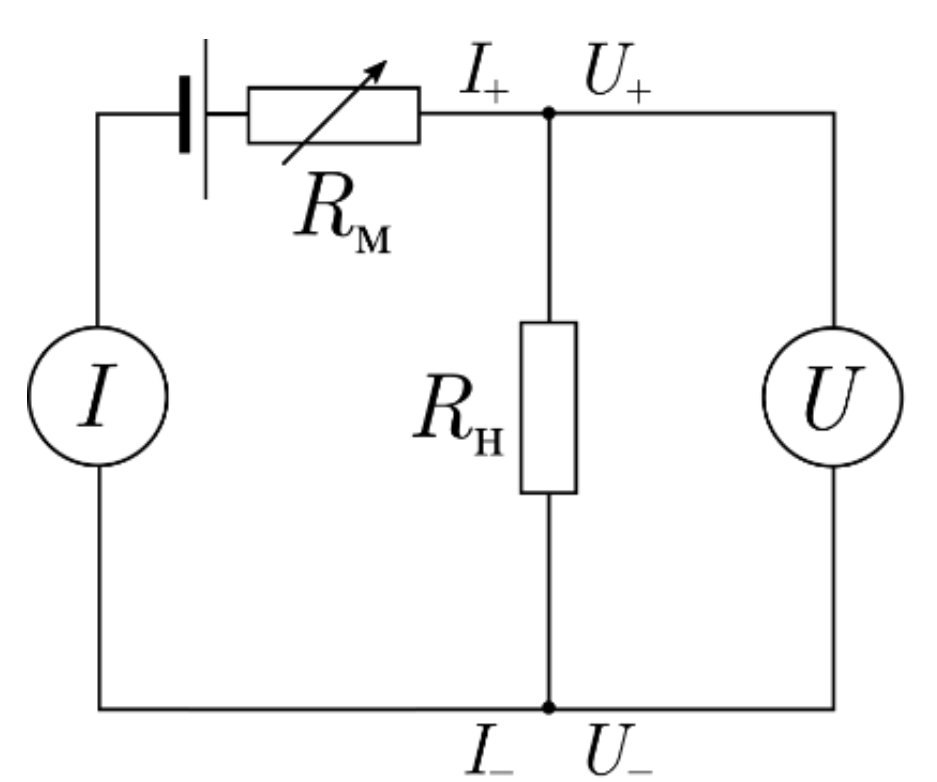
\includegraphics[scale=0.5]{Pictures/Scheme.png}
        \caption{
        рис. 1 Электрическая схема установки
        }
 \end{figure} 
        Сопротивление нити является однозначной функцией её температуры $R (t)$. В исследуемом интервале температур ($20–80 ^\circ C$) зависимость сопротивления от температуры можно с хорошей точностью аппроксимировать линейной функцией:
\begin{equation*}
	R(t) = R_{273} (1+\alpha t),
	\eqno(4)
\end{equation*}
где $t$ - температура в $[^\circ C]$, $R_{273}$ - сопротивление нити при температуре $0 ^\circ C$ и $\alpha = \frac{1}{R_{273}}\frac{dR}{dT}$ - температурный коэффициент сопротивления материала. 

\section{Приборы и данные}
\begin{itemize}
    \item Цифровые мульиметры Вольтметр универсальный B7-78/1, погрешность измерения постоянного тока 0,15\% + 0,02 мА, погрешность измерения постоянного напряжения 0,004\% + 0,007 мВ. 
    \item Термостат Witeg WCR-12, погрешность измерения температуры 0,2 $^\circ C$.
    \item Источник постоянного напряжения GW Instek GPS-2303, погрешность 0,5\% + 10 мВ
    \item Магазин сопротивлений МЕГЕОН05350, погрешность 5\%, 2\%, 1\%, 0,5\% для декад x0,1, x1, x10, x100 соответственно
\end{itemize}

\section{Выполнение}
\begin{enumerate}
\item Проведем предварительные расчеты параметров опыта. Приняв максимально допустимый перегрев нити относительно термостата, а равным $\Delta t_{max} = 30 ^\circ C$ , а коэффициент теплопроводности воздуха $k \approx 25 \frac{\text{мВт}}{\text{м} \cdot \text{K}}$, оценим максимальную мощность нагрева. $Q_{max} = \dfrac{2 \pi L}{\ln \dfrac{r_0}{r_1}} k  \cdot \Delta t_{max} = 381,4 \text{ мВт}$. Сопротивление платиновой нити при комнатной температуре $R_\text{н} \approx 20 \text{ Ом}$. Определим с помощью данных значений значения максимального тока в нити $I_{max}$ и максимального напряжения на ней $U_{max}$.
\begin{equation*}
	U_{max} = \sqrt{Q_{max} R_\text{н}} = 2,76 \text{ В},
\end{equation*}
\begin{equation*}
	I_{max} = \sqrt{\frac{Q_{max}} {R_\text{н}}} = 138,1 \text{ мА}.
\end{equation*}
\item Показания гигрометра: температура у стены с окнами $17 ^\circ C$, влажность 79\%. Температруа термостата $23 ^\circ C$. Проведем первую серию измерений сопротивления нити $R_\text{н} = \frac{U}{I}$ от подаваемой на нее мощности $Q = UI$. Понижая сопротивление на магазине, будем ждать по 30-40 секунд для установления теплового равновесия. Убедимся в том, что зависимость линейная, построив график.\\
По окончании первой серии перведем магазин сопротивления $R_\text{м}$ на 10 кОм, установив минимальный ток через нить. Повысим температуру в термостате и подождем 10-15 минут для установления теплового равновесия в системе. Проделаем этот опыт еще 3 раза для различных температур термостата.
\end{enumerate}
\section{Обработка результатов}
\begin{enumerate}
\item Проведя 4 серии мы получили следующие результаты.
\begin{table}[h!]
    \centering
    \begin{tabular}{|*{9}{c|}}
\hline
        $R_\text{м}, \text{Ом}$ & $I, \text{мА}$ & $U, \text{мВ}$ & $Q, \text{мВт}$ & $\sigma_Q, \text{мВт}$ & $\varepsilon_Q, \%$ & $R, \text{Ом}$ & $\sigma_R,  \text{Ом}$ & $\varepsilon_R, \%$ \\ \hline
        199.9  & 15.70 $\pm$ 0.04 & 308.5  & 4.843  & 0.013  & 0.28  & 19.650  & 0.055  & 0.28 \\ \hline
        99.9   & 28.22 $\pm$ 0.06 & 555.9  & 15.687 & 0.035  & 0.22  & 19.699  & 0.044  & 0.22 \\ \hline
        49.9   & 46.87 $\pm$ 0.09 & 930.6  & 43.617 & 0.084  & 0.19  & 19.855  & 0.038  & 0.19 \\ \hline
        29.9   & 63.54 $\pm$ 0.12 & 1275   & 81.014 & 0.147  & 0.18  & 20.066  & 0.036  & 0.18 \\ \hline
        9.9    & 97.40 $\pm$ 0.17 & 2016.2 & 196.378 & 0.335  & 0.17  & 20.700  & 0.035  & 0.17 \\ \hline
        4.9    & 111.71 $\pm$ 0.19 & 2352.1 & 262.753 & 0.441  & 0.17  & 21.055  & 0.035  & 0.17 \\ \hline
    \end{tabular}
    \caption{Таблица 1. $t = 23,0 ^\circ C$}
\end{table}

\begin{table}[h!]
    \centering
    \begin{tabular}{|*{9}{c|}}
\hline
        $R_\text{м}, \text{Ом}$ & $I, \text{мА}$ & $U, \text{мВ}$ & $Q, \text{мВт}$ & $\sigma_Q, \text{мВт}$ & $\varepsilon_Q, \%$ & $R, \text{Ом}$ & $\sigma_R,  \text{Ом}$ & $\varepsilon_R, \%$ \\ \hline
        199.9  & 16.02 $\pm$ 0.04 & 322.8  & 5.171  & 0.014  & 0.27  & 20.150  & 0.055  & 0.27 \\ \hline
        99.9   & 29.26 $\pm$ 0.06 & 591.5  & 17.307 & 0.038  & 0.22  & 20.215  & 0.044  & 0.22 \\ \hline
        59.9   & 43.68 $\pm$ 0.09 & 888.4  & 38.805 & 0.076  & 0.20  & 20.339  & 0.040  & 0.20 \\ \hline
        39.9   & 57.88 $\pm$ 0.11 & 1186.2 & 68.657 & 0.127  & 0.18  & 20.494  & 0.038  & 0.18 \\ \hline
        19.9   & 85.15 $\pm$ 0.13 & 1783.4 & 151.857 & 0.264  & 0.17  & 20.944  & 0.036  & 0.17 \\ \hline
        9.9    & 110.13 $\pm$ 0.19 & 2369.1 & 260.909 & 0.439  & 0.17  & 21.512  & 0.036  & 0.17 \\ \hline
        6.9    & 120.32 $\pm$ 0.20 & 2622.2 & 315.503 & 0.526  & 0.17  & 21.794  & 0.036  & 0.17 \\ \hline
        3.9    & 132.13 $\pm$ 0.22 & 2929.2 & 387.035 & 0.639  & 0.17  & 22.169  & 0.037  & 0.17 \\ \hline
    \end{tabular}
    \caption{Таблица 2. $t = 30,0 ^\circ C$ }
\end{table}

\begin{table}[h!]
    \centering
    \begin{tabular}{|*{9}{c|}}
\hline
        $R_\text{м}, \text{Ом}$ & $I, \text{мА}$ & $U, \text{мВ}$ & $Q, \text{мВт}$ & $\sigma_Q, \text{мВт}$ & $\varepsilon_Q, \%$ & $R, \text{Ом}$ & $\sigma_R,  \text{Ом}$ & $\varepsilon_R, \%$ \\ \hline
        199.9  & 15.96 $\pm$ 0.04 & 335.1  & 5.348  & 0.015  & 0.28  & 20.996  & 0.058  & 0.28 \\ \hline
        99.9   & 29.06 $\pm$ 0.06 & 612.1  & 17.788 & 0.039  & 0.22  & 21.063  & 0.046  & 0.22 \\ \hline
        59.9   & 43.24 $\pm$ 0.09 & 915.8  & 39.599 & 0.078  & 0.20  & 21.179  & 0.042  & 0.20 \\ \hline
        39.9   & 57.09 $\pm$ 0.11 & 1218.3 & 69.553 & 0.129  & 0.19  & 21.340  & 0.039  & 0.19 \\ \hline
        19.9   & 83.49 $\pm$ 0.13 & 1817.3 & 151.726 & 0.264  & 0.17  & 21.767  & 0.038  & 0.17 \\ \hline
        9.9    & 107.46 $\pm$ 0.18 & 2397.2 & 257.603 & 0.434  & 0.17  & 22.308  & 0.038  & 0.17 \\ \hline
        6.9    & 117.20 $\pm$ 0.20 & 2645.5 & 310.053 & 0.518  & 0.17  & 22.573  & 0.038  & 0.17 \\ \hline
        3.9    & 128.51 $\pm$ 0.22 & 2944.5 & 378.398 & 0.627  & 0.17  & 22.913  & 0.038  & 0.17 \\ \hline
    \end{tabular}
    \caption{Таблица 3. $t = 42,2 ^\circ C$}
\end{table}

\begin{table}[h!]
    \centering
    \begin{tabular}{|*{9}{c|}}
\hline
        $R_\text{м}, \text{Ом}$ & $I, \text{мА}$ & $U, \text{мВ}$ & $Q, \text{мВт}$ & $\sigma_Q, \text{мВт}$ & $\varepsilon_Q, \%$ & $R, \text{Ом}$ & $\sigma_R,  \text{Ом}$ & $\varepsilon_R, \%$ \\ \hline
        199.9  & 15.87 $\pm$ 0.04 & 352.2  & 5.589  & 0.015  & 0.28  & 22.193  & 0.061  & 0.28 \\ \hline
        99.9   & 28.78 $\pm$ 0.06 & 640.4  & 18.431 & 0.040  & 0.22  & 22.252  & 0.049  & 0.22 \\ \hline
        59.9   & 42.62 $\pm$ 0.09 & 953.1  & 40.621 & 0.080  & 0.20  & 22.363  & 0.044  & 0.20 \\ \hline
        39.9   & 56.03 $\pm$ 0.11 & 1261.4 & 70.676 & 0.131  & 0.19  & 22.513  & 0.042  & 0.19 \\ \hline
        19.9   & 81.29 $\pm$ 0.13 & 1862.6 & 151.411 & 0.264  & 0.17  & 22.913  & 0.040  & 0.17 \\ \hline
        9.9    & 103.95 $\pm$ 0.18 & 2433.4 & 252.952 & 0.428  & 0.17  & 23.409  & 0.040  & 0.17 \\ \hline
    \end{tabular}
    \caption{Таблица 4. $t = 59,0 ^\circ C$}
\end{table}
\clearpage
\item Построим по методу наименьших квадратов график зависимости сопротивления нити от мощности $R(Q)$.

\begin{figure}[h!]
\centering{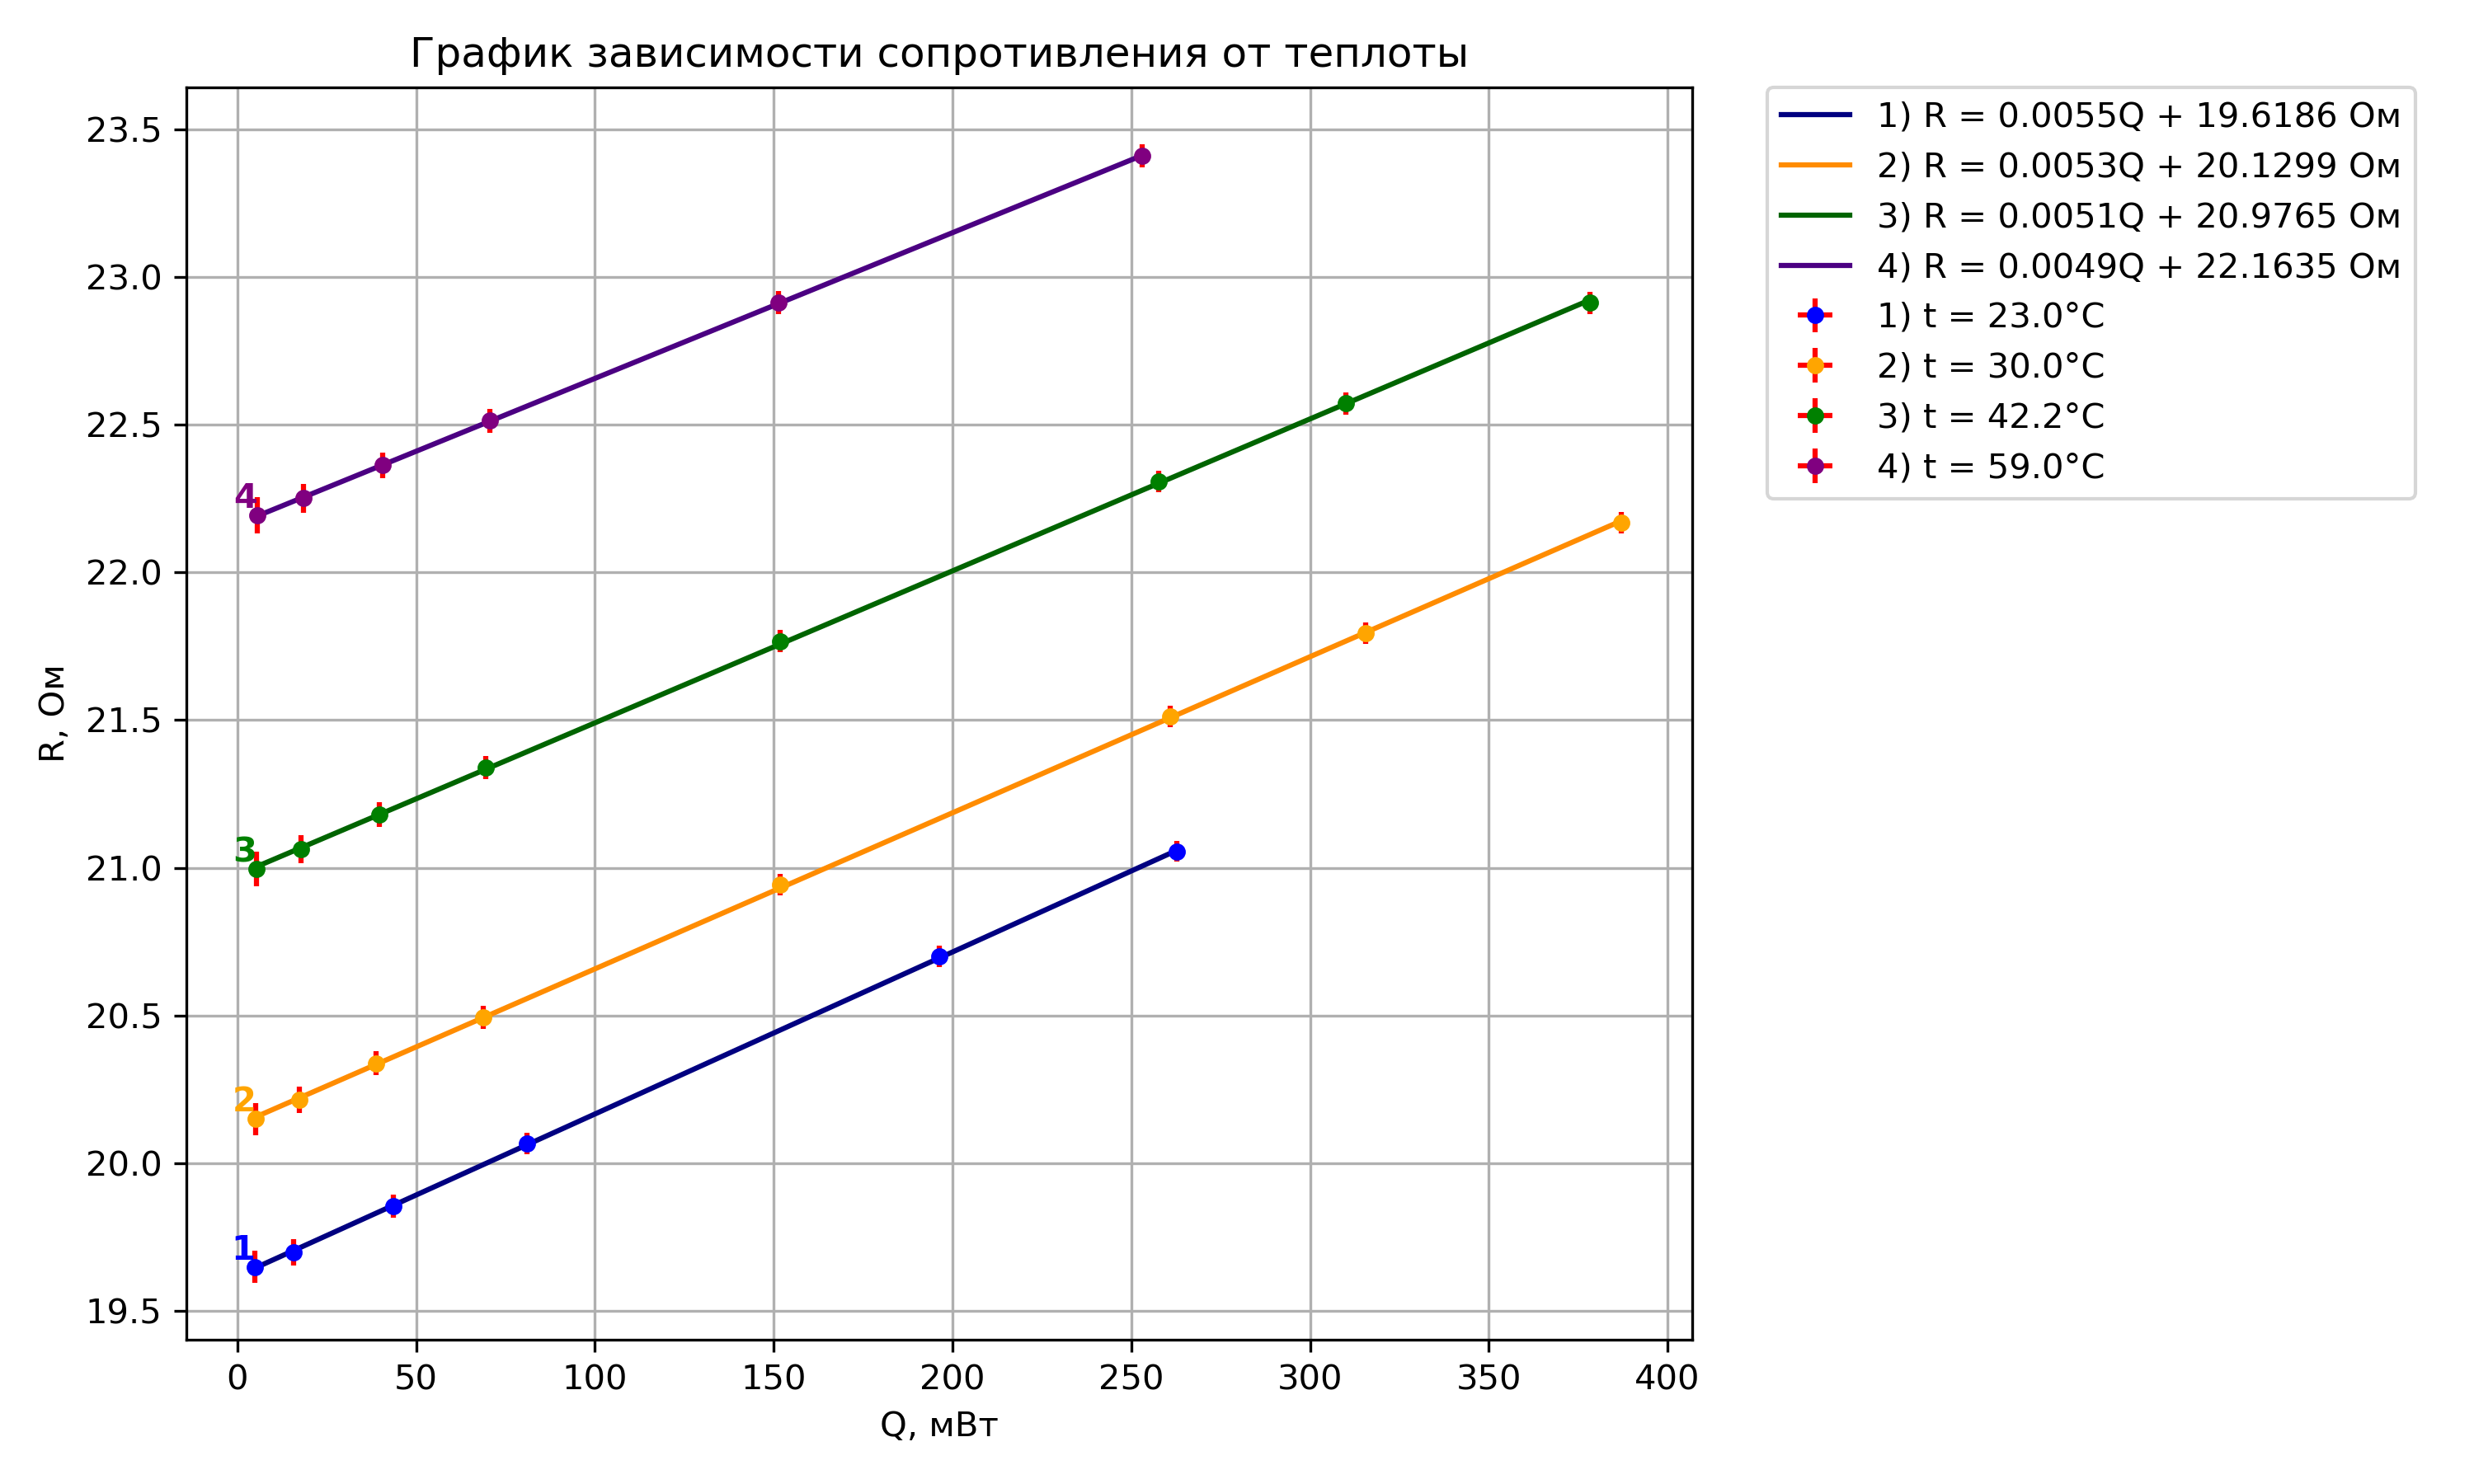
\includegraphics[width=1\textwidth]{Graphics/graph11.png}}
\caption[]{\label{} График №1 Зависимость $R(Q)$}
\end{figure}

Из графика видно, что зависимость линейная. Определим сопротивление нити при $Q \rightarrow 0$ $R_0$ и угловые коэффициенты $\frac{dR}{dQ}$ для исследуемых температур.

\begin{table}[h!]
    \centering
    \begin{tabular}{|*{7}{c|}}
\hline
        $T, ^\circ C$ & $\frac{dR}{dQ},  \frac{\text{Ом}}{\text{Вт}}$ & $\sigma_{\frac{dR}{dQ}}, \frac{\text{Ом}}{\text{Вт}}$ & $\varepsilon_{\frac{dR}{dQ}}, \%$ &$R_0, \text{Ом}$ & $\sigma_{R_0}, \text{Ом}$ & $\varepsilon_{R_0}, \%$ \\ \hline
        23.0  $\pm$ 0.2 & 5.483  & 0.018  & 0.33  & 19.6186  & 0.0018  & 0.009 \\ \hline
        30.0  $\pm$ 0.2 & 5.282  & 0.016  & 0.30  & 20.1299  & 0.0022  & 0.011 \\ \hline
        42.2 $\pm$ 0.2& 5.143  & 0.017  & 0.34  & 20.9765  & 0.0024  & 0.011 \\ \hline
        59.0  $\pm$ 0.2 & 4.932  & 0.009  & 0.19  & 22.1635  & 0.0008  & 0.004 \\ \hline
    \end{tabular}
    \caption{Таблица 5. Сопротивления $R_0$ и коэффициенты $\frac{dR}{dQ}$ для исследуемых температур}
\end{table}

\item Пользуясь полученными значениями $R_0$ построим по МНК график зависимости сопротивления нити от температуры $R(T)$.
\clearpage
\begin{figure}[h!]
\centering{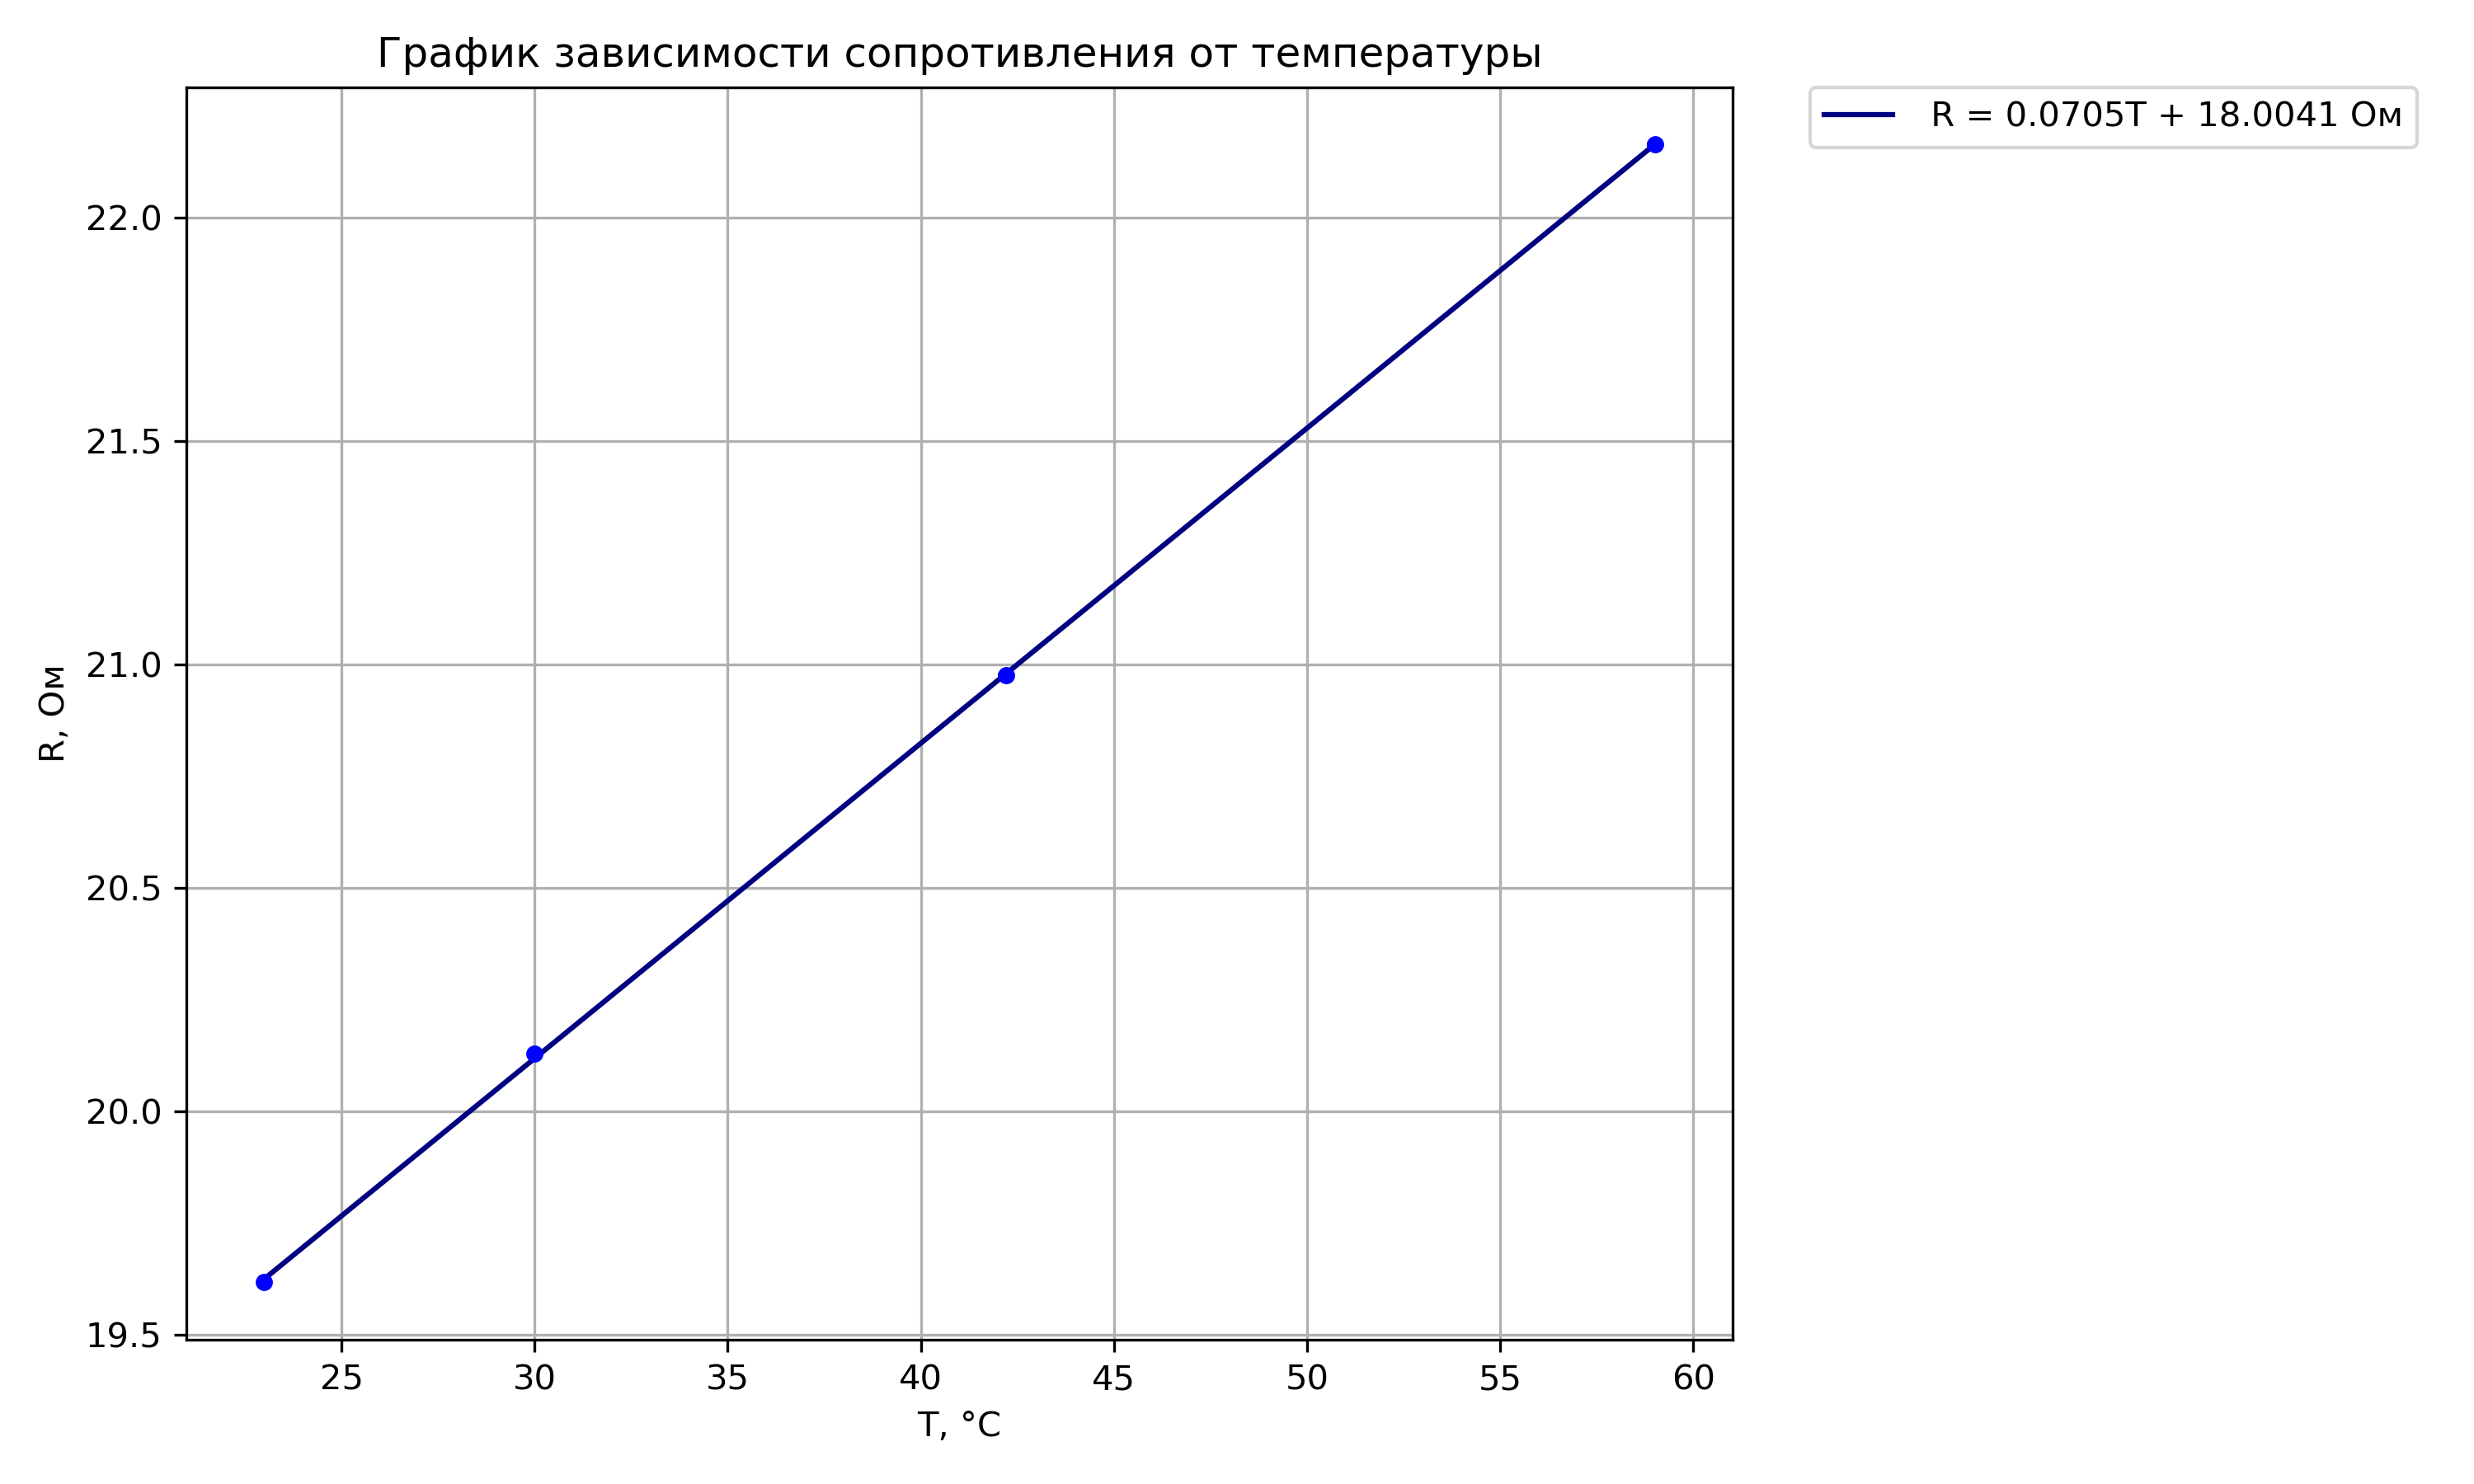
\includegraphics[width=1\textwidth]{Graphics/graph12.png}}
\caption[]{\label{} График №2 Зависимость $R(T)$}
\end{figure}

Из графика видно, что зависимость линейная. Определим наклон прямой $\frac{dR}{dT}$, сопротивление при $0 ^\circ C$ $R_{273}$ и температурный коэффициент сопротивления материала нити $\alpha$.
\begin{equation*}
	\frac{dR}{dT} = (7,05 \pm 0,02) \cdot 10^{-2} \frac{\text{Ом}}{\text{К}} (\varepsilon_{\frac{dR}{dT}} = 0,34\%),
\end{equation*}
\begin{equation*}
	R_{273} = 18,004 \pm 0,003 \text{Ом} (\varepsilon_{R_{273}} = 0,02\%),
\end{equation*}
\begin{equation*}
	\alpha = \frac{1}{R_{273}}\frac{dR}{dT} = 3,916 \pm 0,013, 10^{-3} \text{К}^{-1} (\varepsilon_{\alpha} = 0,34\%),
\end{equation*}

Значение $\alpha$ довольно близко к табличному значению для платины ($\alpha_{Pt} ^{\text{табл}} = 3,8 \cdot 10^{-3} \text{К}^{-1} $).

\item Найдем коэффициенты теплопроводности воздуха при атмосферном давлении для наших температур:
\begin{equation*}
	k = \frac{dQ}{dT} \frac{ln\frac{r_o}{r_1}}{2\pi L} = \frac{\frac{dR}{dT}}{\frac{dR}{dQ}} \frac{ln\frac{r_o}{r_1}}{2\pi L}
\end{equation*}

\begin{table}[h!]
    \centering
    \begin{tabular}{|*{4}{c|}}
	\hline
        $T, ^\circ C$ & $k, \frac{\text{мВт}}{\text{м} \cdot \text{K}}$ & $\sigma_k,  \frac{\text{мВт}}{\text{м} \cdot \text{K}}$& $\varepsilon_k$, \% \\ \hline
        23.0 $\pm$ 0.2  & 25.28 & 0.42 & 1.65 \\ \hline
        30.0 $\pm$ 0.2  & 26.24 & 0.43 & 1.65 \\ \hline
        42.2 $\pm$ 0.2& 26.96 & 0.45 & 1.66 \\ \hline
        59.0  $\pm$ 0.2 & 28.11 & 0.46 & 1.63 \\ \hline
    \end{tabular}
    \caption{Таблица 6. Коэффициенты теплопроводности воздуха\\ при атмосферном давлении для исследуемых температур}
\end{table}

\item Построим график зависимости теплопроводности воздуха от температуры газа k(T) в обычном и в двойном логарифмическом масштабах.

\begin{figure}[h!]
\centering{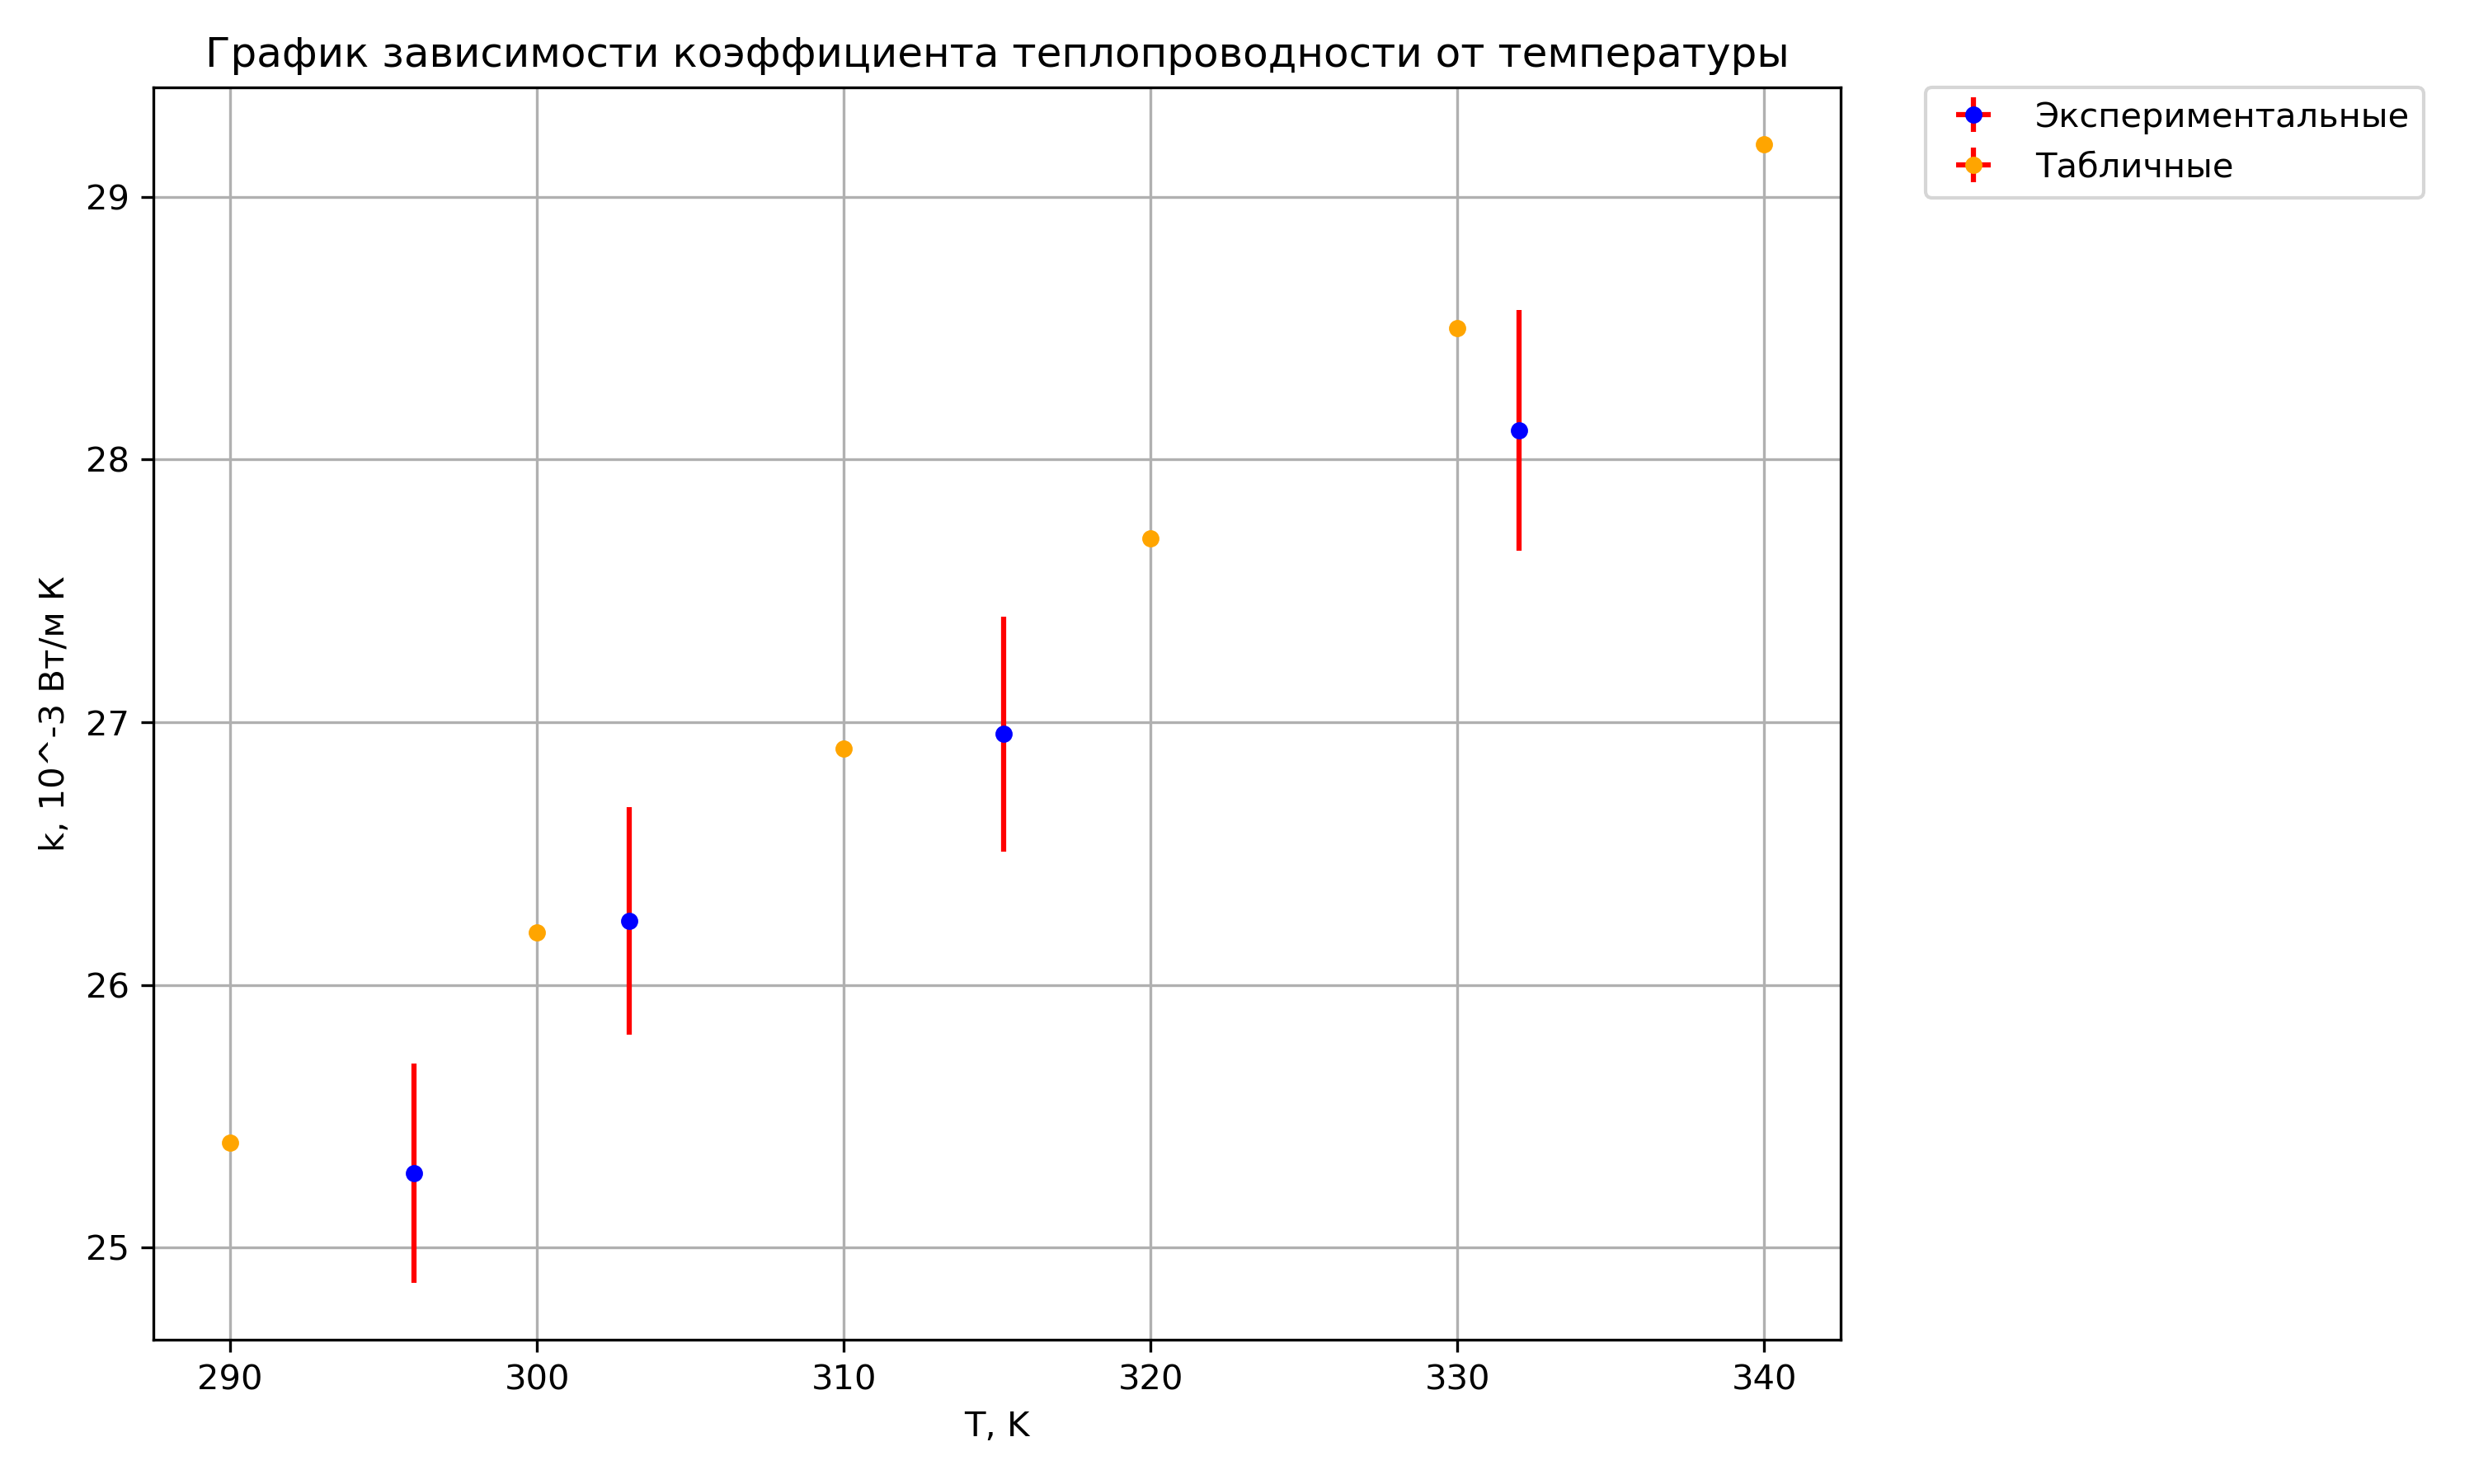
\includegraphics[width=1\textwidth]{Graphics/graph14.png}}
\caption[]{\label{} График №3 Зависимость $k(T)$}
\end{figure}

\begin{figure}[h!]
\centering{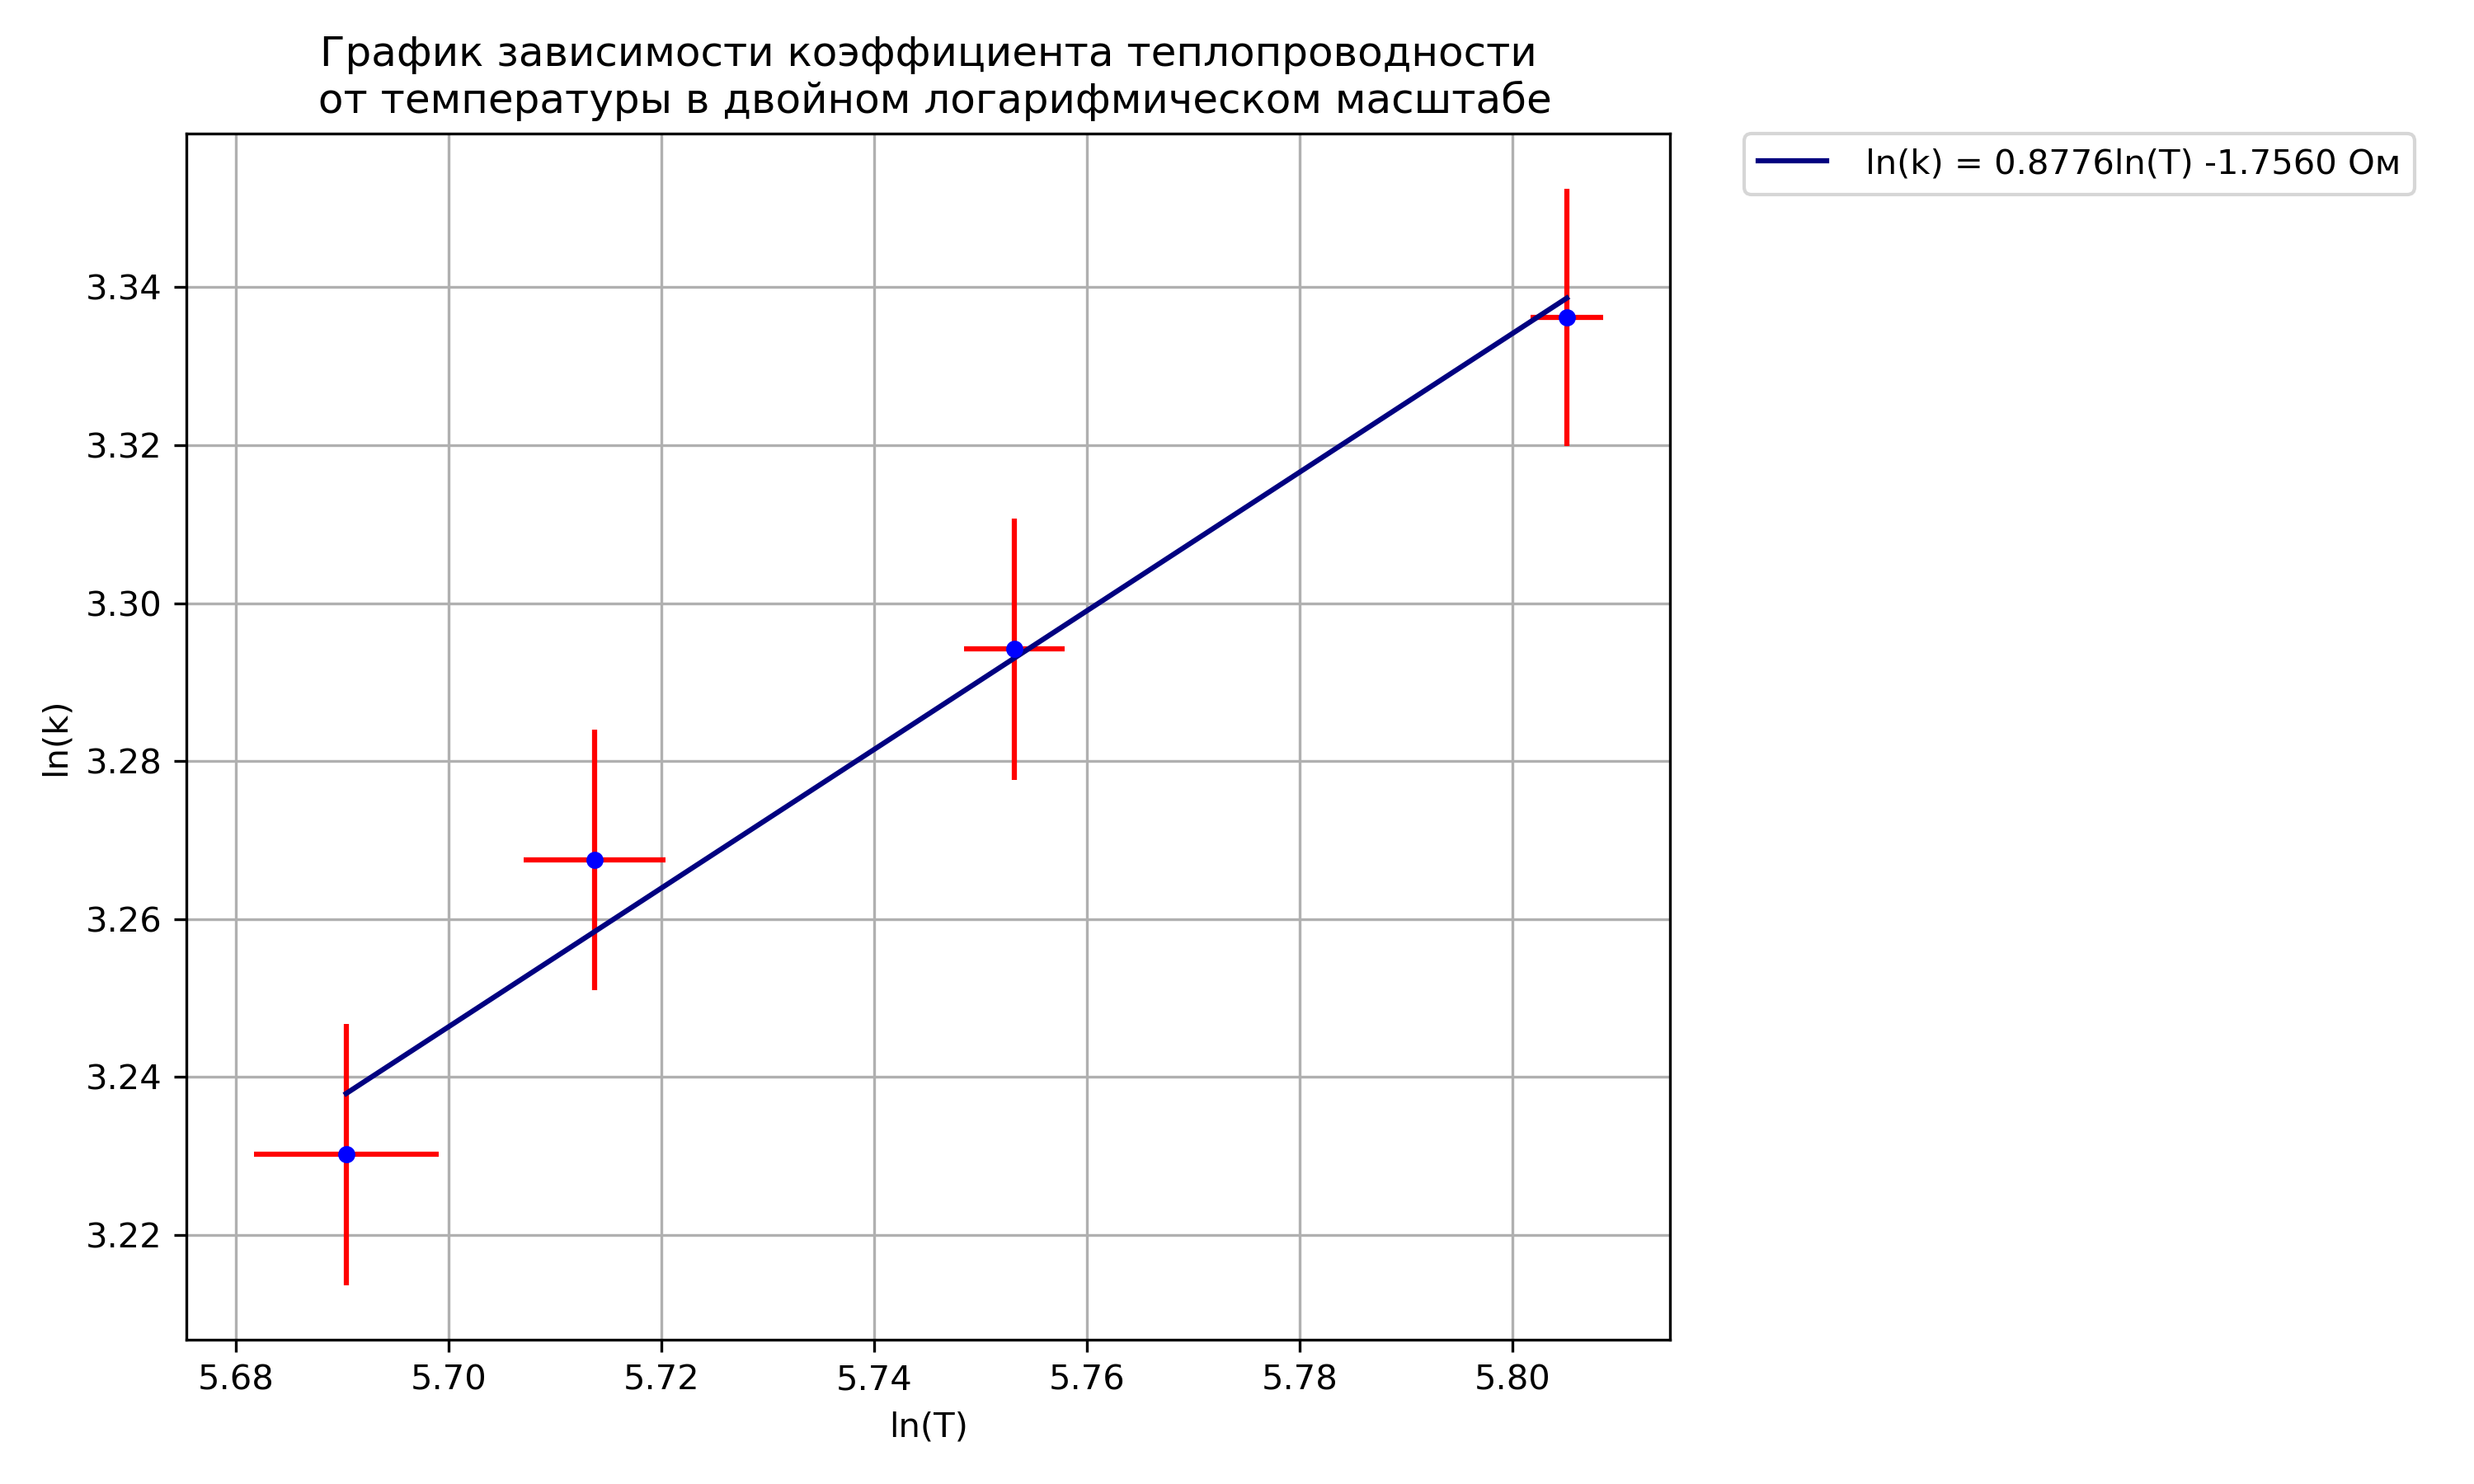
\includegraphics[width=1\textwidth]{Graphics/graph13.png}}
\caption[]{\label{} График №4 Зависимость $k(T)$ в двойном логарифмическом масштабе}
\end{figure}
\clearpage
Предполагая, что коэффициент теплопроводности воздуха зависит степенным образом от абсолютной температуры: $k \sim T^\beta$, вычислим по графику №4 $\beta = 0,88 \pm 0,07 (\varepsilon_\beta = 7,98 \%)$. Теоретический коэффициет равен 0.5, поскольку $k \sim \lambda \overline{\nu} \cdot n c_V \label{k}$, где $\overline{\nu} = \sqrt{\frac{8k_{\text{Б}}T}{\pi m}}$.


\section{Результаты и обсуждения}
Сравним полученные экспериментально значения коэффициента теплопроводности воздуха при атмосферном давлении для исследуемых температур с табличными значениями. В таблице приведены вычисленные на основе данных из книги Лабораторный практикум по общей физике Том 1 Термодинамика и молекулярная физика коэффициента по линейной зависимости ($k = aT + b$) и степенной с показателем $\frac{1}{2}$ ($k = \alpha \sqrt{T} + \beta$).
\begin{table}[h!]
    \centering
    \begin{tabular}{|*{10}{c|}}
	\hline
        $T, K$ & $k_\text{эксп}, \frac{\text{мВт}}{\text{м} \cdot \text{K}}$ & $k_{\text{теор}}^{\text{line}}, \frac{\text{мВт}}{\text{м} \cdot \text{K}}$ & $k_{\text{теор}}^{\text{root}}, \frac{\text{мВт}}{\text{м} \cdot \text{K}}$ & $\sigma_{\text{эксп}}, \frac{\text{мВт}}{\text{м} \cdot \text{K}}$ & $\sigma_{\text{теор}}^{\text{line}}, \frac{\text{мВт}}{\text{м} \cdot \text{K}}$ & $\sigma_{\text{теор}}^{\text{root}}, \frac{\text{мВт}}{\text{м} \cdot \text{K}}$ & $\varepsilon_{\text{эксп}}, \%$ & $\varepsilon_{\text{теор}}^{\text{line}}, \%$ & $\varepsilon_{\text{теор}}^{\text{root}}, \%$ \\ \hline
        296.0 $\pm$ 0.2  & 25.28 & 25.88 & 25.88 & 0.42 & 0.60 & 0.60 & 1.65 & 2.30 & 2.31 \\ \hline
        303.0 $\pm$ 0.2  & 26.24 & 26.41 & 26.41 & 0.43 & 0.17 & 0.17 & 1.65 & 0.63 & 0.63 \\ \hline
        315.2 $\pm$ 0.2 & 26.96 & 27.32 & 27.31 & 0.45 & 0.36 & 0.36 & 1.66 & 1.32 & 1.30 \\ \hline
        332.0 $\pm$ 0.2 & 28.11 & 28.64 & 28.66 & 0.46 & 0.53 & 0.55 & 1.63 & 1.85 & 1.91 \\ \hline
    \end{tabular}
    \caption{Таблица 7. Сравнение экспериментальных и табличных значений}
\end{table}

Как мы видим, полученные значения с хорошей точностью совпадают с табличными. Также можно отметить, что расхождение между степенной и линейной зависимостью минимальны, что означает, что полученный по графику №4 показатель $\beta$, несмотря на сильное расхождение с теоретическим, для данного диапазона не сильно влияет на точность полученных значений. Стоит отметить, что эффективное сечение столкновение $\sigma$ является медленно убывающей функцией $T$, поэтому по соотношению (2) можно сделать вывод, что показатель $\beta$ должен быть больше $\frac{1}{2}$.

\end{enumerate}

\section{Выводы}
\begin{enumerate}
\item В данной работе были измерены зависимости сопротивления платиновой нити от подаваемой на нее мощности при разных температурах. Построены графики зависимостей $R(Q)$, получены угловые коэффициенты $\frac{dR}{dQ}$ и сопротивления нити при данных температурах (при $Q \rightarrow 0$). Относительная погрешность величин мала из-за высокой точности приборов (в частности мультиметров)
\item при помощи полученных сопротивлений построили график зависимости сопротивления нити от ее температуры $R(T)$, вычислили температурный коэффициент сопротивления платиновой нити. $\alpha_{\text{эксп}} =  3,916 \pm 0,013, 10^{-3} \text{К}^{-1}$ $(\varepsilon_{\alpha} = 0,34\%)$,  $\alpha_{\text{табл}} = 3,8 \cdot 10^{-3} \text{К}^{-1}$. Значения отличаются на $0,116 \cdot 10^{-3} \text{К}^{-1} (\varepsilon = 3,05 \%)$, поэтому экспериментальная величина довольна близка к табличной.
\item Вычислили коэффициенты теплопроводности воздуха при атмосферном давлении и разных температурах. Табличные значения для температур $t_2 = 30,0 ^\circ C$ и $t_3 = 42,2 ^\circ C$ с большим числом измеренных точек зависимости $R(Q)$ входят в диапазон погрешности экспериментальных. Относительная погрешность коэффициента для каждой температуры не превосходит $1,66 \%$ (см. таблицу 7).
\item Предположив, что коэффициент теплопроводности зависит от температуры степенным образом, по графику зависимости $lnk(lnT)$ определили показатель. $\beta_{\text{эксп}} = 0,88 \pm 0,07 (\varepsilon_\beta = 7,98 \%)$, $\beta_{\text{теор}} = 0,5$. Значения сильно отличаются, однако исходя из таблицы 7, можно сделать вывод, что при показателе от 0,5 до 1 экспериментальные и теоретические значения rкоэффициентов теплопроводности не сильно расходятся.
\end{enumerate}

\end{document}